%
%===============>>  ГРУППА 8-2 МОДУЛЬ 8  <<=============
%
\setmodule{8}

%BEGIN_FOLD % ====>>_____ Занятие 1 _____<<====
\begin{class}[number=1]
	\begin{listofex}
		\item Решите уравнения:
		\begin{tasks}(2)
			\task \( x^4-20x^2+64=0 \)
			\task \( (x^2+x)^2-8x^2-8x+12=0 \)
		\end{tasks}
		\item Решите уравнения:
		\begin{tasks}(2)
			\task \( \dfrac{x^2-x}{x^2-x+1}-\dfrac{x^2-x+2}{x^2-x-2}=1 \)
			\task \( \dfrac{2x-1}{x}+\dfrac{4x}{2x-1}=5 \)
			\task! \( \dfrac{4}{9x^2-9x+2}-\dfrac{8}{9x^2-9x+8}=1 \)
		\end{tasks}
		\item Решите уравнения:
		\begin{tasks}(2)
			\task \( x^2-7|x|-8=0 \)
			\task \( (x^2-4)|x|+3=0 \)
			\task \( (x-7)^2-|x-7|=30 \)
			\task \( (x-2)^2+2|x-2|-8=0 \)
		\end{tasks}
	\end{listofex}
\end{class}
%END_FOLD

%BEGIN_FOLD % ====>>_____ Занятие 2 _____<<====
\begin{class}[number=2]
	\begin{listofex}
		\item Решите биквадратное уравнение:
		\begin{tasks}(2)
			\task \( 4x^4-41x^2+100=0 \)
			\task \( 6c^4-35=11c^2 \)
			\task \( 10p^4-21=p^2 \)
			\task \( x^4+4x^2-21=0 \)
		\end{tasks}
		\item Решите уравнения:
		\begin{tasks}(2)
			\task \( (2x^2+3)^2-12(2x^2+3)+11=0 \)
			\task \( (x^2+3)^2-11(x^2+3)+28=0 \)
			\task \( (x^2-4x)^2+9(x^2-4x)+20=0 \)
			\task \( (t^2-2t)^2-3=2(t^2-2t) \)
			\task \( (x^2+x-1)(x^2+x+2)=40 \)
			\task \( (2x^2+x-1)(2x^2+x-4)+2=0 \)
		\end{tasks}
	\end{listofex}
\end{class}
%END_FOLD

%BEGIN_FOLD % ====>>_ Домашняя работа 1 _<<====
\begin{homework}[number=1]
	\begin{listofex}
		\item Решите биквадратные уравнения:
		\begin{tasks}(2)
			\task \( 9x^4=9x^2-1 \)
			\task \( 3x^4+21=4x^2 \)
		\end{tasks}
		\item Решите уравнения:
		\begin{tasks}(2)
			\task \( (2x+3)^2=3(2x+3)-2 \)
			\task \( (x^2-2x)^2-4(x^2-2x)+3=0 \)
			\task! \( (x^2+x)(x^2+x-5)=84 \)
		\end{tasks}
		\item Теплоход проходит по течению реки до пункта назначения \( 280 \) км и после стоянки возвращается в пункт отправления. Найдите скорость теплохода в неподвижной воде, если скорость течения равна \( 4 \) км/ч, стоянка длится \( 15 \) часов, а в пункт отправления теплоход возвращается через \( 39 \) часов после отплытия из него.
	\end{listofex}
\end{homework}
%END_FOLD

%BEGIN_FOLD % ====>>_____ Занятие 3 _____<<====
\begin{class}[number=3]
	\begin{listofex}
		\item Решите уравнения:
		\begin{tasks}(2)
			\task \( x^2-7|x|-8=0 \)
			\task \( (x^2-4)|x|+3=0 \)
			\task \( (x-7)^2-|x-7|=30 \)
			\task \( (x-2)^2+2|x-2|-8=0 \)
		\end{tasks}
		\item Решите системы уравнений:
		\begin{itasks}[2]
			\task \exercise{191}
			\task \exercise{190}
			\task \exercise{206}
			\task \exercise{207}
			\task \exercise{219}
			\task \exercise{220}
		\end{itasks}
		\item Решите уравнение: \[ 7\left( x+\dfrac{1}{x} \right)+2\left( x^2+\dfrac{1}{x^2} \right)+9=0 \]
	\end{listofex}
\end{class}
%END_FOLD

%BEGIN_FOLD % ====>>_____ Занятие 4 _____<<====
\begin{class}[number=4]
	\begin{listofex}
		\item Решите системы уравнений:
		\begin{itasks}[2]
			\task \exercise{192}
			\task \exercise{193}
			\task \exercise{194}
			\task \exercise{195}
			\task \exercise{208}
			\task \exercise{209}
			\task \exercise{210}
			\task \exercise{211}
		\end{itasks}
		\item Мать старше дочери на \( 23 \) года, а вместе им \( 51 \) год. Сколько лет дочери?
		\item Девять лет назад брат был вдвое старше сестры. Сколько лет брату и сколько сестре, если брат старше сестры на \( 4 \) года?
		\item Моторная лодка за \( 3 \) часа движения против течения реки и \( 2,5 \) часа по течению проходит \( 98 \) км. Найдите собственную скорость лодки и скорость течения, если за \( 5 \) часов движения по течению она проходит на \( 36 \) км больше, чем за \( 4 \) часа против течения реки.
		\item Вкладчик положил в банк \( 21000 \) р. на два разных счета. По первому из них	банк выплачивает \( 4\% \) годовых, а по второму --- \( 6\% \) годовых. Через год вкладчик получил по процентам \( 1020 \) р. Сколько рублей он положил на каждый счет?
		\item Разность двух натуральных чисел равна \( 48 \) Если первое число разделить на второе, то в частном получится \( 4 \), а в остатке \( 3 \). Найдите эти числа.
		\item Имеется два сплава меди и цинка. Один сплав содержит \( 9\% \), а другой --- \( 30\% \) цинка. Сколько килограммов каждого сплава надо взять, чтобы получить сплав массой \( 300 \) кг, содержащий \( 23\% \) цинка?
	\end{listofex}
\end{class}
%END_FOLD

%BEGIN_FOLD % ====>>_ Домашняя работа 2 _<<====
\begin{homework}[number=2]
	\begin{listofex}
		\item Решите системы уравнений:
		\begin{itasks}[2]
			\task \exercise{197}
			\task \exercise{199}
			\task \exercise{212}
			\task \exercise{214}
		\end{itasks}
		\item Вкладчик положил в банк \( 30000 \) р. на два разных счета. По первому из них банк выплачивает \( 5\% \) годовых, а по второму --- \( 7\% \) годовых. Через год вкладчик получил по первому вкладу на \( 60 \) р. процентных денег больше, чем по второму вкладу. Сколько рублей он положил на каждый счет?
		\item Сумма цифр двузначного числа равна \( 15 \). Если поменять его цифры местами, то получим число, которое меньше данного на \( 9 \). Найдите данное число.
		\item Имеется два водно-солевых раствора. Первый раствор содержит \( 25\% \), а	второй --- \( 40\% \) соли. Сколько килограммов раствора надо взять, чтобы получить \( 50 \) кг раствора, содержащего \( 34\% \) соли?
	\end{listofex}
\end{homework}
%END_FOLD

%BEGIN_FOLD % ====>>_____ Занятие 5 _____<<====
\begin{class}[number=5]
	\begin{listofex}
		\item Занятие 5
	\end{listofex}
\end{class}
%END_FOLD

%BEGIN_FOLD % ====>>_____ Занятие 6 _____<<====
\begin{class}[number=6]
	\begin{listofex}
		\item Занятие 6
	\end{listofex}
\end{class}
%END_FOLD

%BEGIN_FOLD % ====>>_ Домашняя работа 3 _<<====
\begin{homework}[number=3]
	\begin{listofex}
		\item Домашняя работа 3
	\end{listofex}
\end{homework}
%END_FOLD

%BEGIN_FOLD % ====>>_____ Занятие 7 _____<<====
\begin{class}[number=7]
	\title{Подготовка к проверочной}
	\begin{listofex}
		\item Занятие 7
	\end{listofex}
\end{class}
%END_FOLD

%BEGIN_FOLD % ====>>_ Проверочная работа _<<====
\begin{exam}
	\begin{listofex}
		\item 
	\end{listofex}
\end{exam}
%END_FOLD

%BEGIN_FOLD % ====>>_____ Консультация 1 _____<<====
\begin{consultation}[number=1]
	\begin{listofex}
		\item 
		\begin{minipage}[t]{\bodywidth}
			Назовите числовой отрезок
		\end{minipage}
		\hspace{0.02\linewidth}
		\begin{minipage}[t]{\picwidth}
			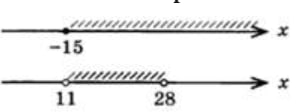
\includegraphics[align=t, width=\linewidth]{\picpath/82M8CONS-1}
		\end{minipage}
		\item 
		\begin{minipage}[t]{\bodywidth}
			Назовите числовой отрезок
		\end{minipage}
		\hspace{0.02\linewidth}
		\begin{minipage}[t]{\picwidth}
			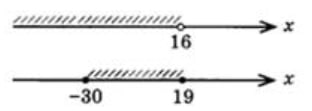
\includegraphics[align=t, width=\linewidth]{\picpath/82M8CONS-2}
		\end{minipage}
		\item Принадлежат ли промежутку \( (-1,8;1,6) \) числа : \( -2 \), \( -1,5 \), \( -1,3 \), \( 0 \), \( 1,4 \), \( 1,6 \)
		\item Изобразите на координатной прямой числовой промежуток, и назовите его:
		\begin{tasks}(3)
			\task \( [3;6] \)
			\task \( (-3;9] \)
			\task \( (-\infty;-6] \)
			\task \( [-5;+\infty) \)
			\task \( [4;16) \)
			\task \( (-\infty;+\infty )\)
		\end{tasks}
		\item Найти пересечение числовых промежутков, используя координатную прямую.
		\begin{tasks}(1)
			\task \( [-2;8] \) и \( (-3;6] \)
			\task \( [-9;3] \) и \( [-5;5] \)
			\task \( (-\infty;-5] \) и \( (-5;+\infty) \)
		\end{tasks}
		\item Найти объединение числовых промежутков, используя координатную прямую.
		\begin{tasks}(1)
			\task \( (-5;2) \) и \( (-2;7] \)
			\task \( [-10;2] \) и \( [-1;10] \)
			\task \( (-\infty;-3] \) и \( (0;+\infty) \)
		\end{tasks}
		\item Изобразите на числовом промежутке:
		\begin{tasks}(2)
			\task \( 2\leq x\leq 10\)
			\task \( -1< x\leq 0\)
			\task \( -\infty < x< 4\)
			\task \( -2\leq x<+\infty \)
		\end{tasks}
		\item Решите неравенства:
		\begin{tasks}(2)
			\task \( x+4<-3 \)
			\task \( x-9\leq 1 \)
			\task \( x>5x-2\)
			\task \( x-4\geq 2x+8\)
		\end{tasks}
	\end{listofex}
\end{consultation}
%END_FOLD